\documentclass[12pt,a4paper]{article}
% =====================================================================
%  BrewLite -- shared preamble for the Assignment reports
%  Compile with pdfLaTeX (TeX Live 2026, vntex + T5 for Vietnamese)
% =====================================================================
\usepackage[utf8]{inputenc}
\usepackage[T5]{fontenc}
\usepackage[utf8]{vntex}

\usepackage[margin=2.2cm,top=2.4cm,bottom=2.2cm,headheight=15pt,footskip=12mm]{geometry}

\usepackage{graphicx}
\usepackage{array}
\usepackage{tabularx}
\usepackage{booktabs}
\usepackage{multirow}
\usepackage{longtable}
\usepackage{amsmath,amssymb}
\usepackage{fancyhdr}
\usepackage{lastpage}
\usepackage{setspace}
\usepackage{enumitem}
\usepackage{float}
\usepackage[table]{xcolor}
\usepackage{tikz}
\usetikzlibrary{arrows.meta,positioning,fit,shapes.geometric,calc,backgrounds}
\usepackage{caption}
\usepackage{titlesec}
\usepackage{microtype}
\usepackage{needspace}
\usepackage{listings}
\usepackage[most]{tcolorbox}
\usepackage[hidelinks]{hyperref}

% ---------------------------------------------------------------------
%  Palette
% ---------------------------------------------------------------------
\definecolor{coffee}{HTML}{6F4E37}
\definecolor{latte}{HTML}{C08552}
\definecolor{cream}{HTML}{F6F1E7}
\definecolor{ink}{HTML}{2B2118}
\definecolor{mint}{HTML}{2F6B4F}
\definecolor{brick}{HTML}{9B2C2C}

% ---------------------------------------------------------------------
%  Layout
% ---------------------------------------------------------------------
\setstretch{1.10}
\setlength{\parindent}{0pt}
\setlength{\parskip}{3.5pt}
\setlength{\emergencystretch}{3em}
\renewcommand{\arraystretch}{1.12}
\setlength{\tabcolsep}{5.5pt}
\setlist{nosep,leftmargin=1.2em,topsep=3pt}
\setcounter{secnumdepth}{2}
\setcounter{tocdepth}{2}

\captionsetup{font=small,labelfont={bf,color=coffee},justification=centering,
  skip=5pt,width=0.94\textwidth}
\captionsetup[table]{position=top,skip=4pt}

% ---------------------------------------------------------------------
%  Headings
% ---------------------------------------------------------------------
\titleformat{\section}
  {\normalfont\Large\bfseries\color{coffee}}
  {\thesection.}{0.5em}{}
  [\vspace{-6pt}{\color{latte}\rule{\textwidth}{1pt}}]
\titleformat{\subsection}
  {\normalfont\large\bfseries\color{ink}}
  {\thesubsection}{0.5em}{}
\titlespacing*{\section}{0pt}{8pt}{4pt}
\titlespacing*{\subsection}{0pt}{8pt}{3pt}

% ---------------------------------------------------------------------
%  Header / footer
% ---------------------------------------------------------------------
\newcommand{\RunningHead}{BrewLite}
\pagestyle{fancy}
\fancyhf{}
\renewcommand{\headrulewidth}{0.4pt}
\renewcommand{\footrulewidth}{0pt}
\fancyhead[L]{\footnotesize\color{coffee}\RunningHead}
\fancyhead[R]{\footnotesize\color{coffee}\thepage\,/\,\pageref{LastPage}}
\fancyfoot[C]{\footnotesize\color{coffee!70}Khoa Công nghệ Thông tin -- Trường Đại học Sài Gòn}

% ---------------------------------------------------------------------
%  Listings (code is ASCII only -- Vietnamese stays in prose)
% ---------------------------------------------------------------------
\lstdefinestyle{bl}{
  basicstyle=\ttfamily\scriptsize,
  keywordstyle=\color{coffee}\bfseries,
  commentstyle=\color{mint}\itshape,
  stringstyle=\color{brick},
  numbers=left, numberstyle=\tiny\color{latte}, numbersep=6pt,
  frame=single, rulecolor=\color{latte!60},
  backgroundcolor=\color{cream},
  breaklines=true, showstringspaces=false,
  xleftmargin=14pt, framexleftmargin=12pt,
  aboveskip=4pt, belowskip=3pt, columns=fullflexible
}

% ---------------------------------------------------------------------
%  Small helpers
% ---------------------------------------------------------------------
\newcommand{\code}[1]{\texttt{\small #1}}
\newcommand{\file}[1]{\texttt{\footnotesize #1}}
\newcommand{\good}[1]{\textcolor{mint}{\textbf{#1}}}
\newcommand{\bad}[1]{\textcolor{brick}{\textbf{#1}}}
\newcommand{\figref}[1]{Hình~\ref{#1}}
\newcommand{\tabref}[1]{Bảng~\ref{#1}}

% Callout box: \begin{note} ... \end{note}
\newtcolorbox{note}[1][Ghi chú]{
  colback=cream, colframe=latte!70, boxrule=0.6pt, arc=2pt,
  left=7pt, right=7pt, top=5pt, bottom=5pt,
  fonttitle=\footnotesize\bfseries, coltitle=coffee,
  title={#1}, fontupper=\footnotesize, before skip=5pt, after skip=5pt
}

% Compact verdict badge used in the NFR table
\newcommand{\pass}{\textcolor{mint}{\textbf{Đạt}}}
\newcommand{\partialok}{\textcolor{latte}{\textbf{Đạt một phần}}}

% ---------------------------------------------------------------------
%  Cover (fields are overridable from each report)
% ---------------------------------------------------------------------
\newcommand{\ReportKind}{Assignment 1}
\newcommand{\ReportTitle}{BrewLite}
\newcommand{\ReportSubtitle}{Nền tảng đặt cà phê trực tuyến\\ thanh toán không dùng tiền mặt}
\newcommand{\CourseName}{Phát triển ứng dụng Web}
\newcommand{\LecturerName}{Từ Lãng Phiêu}
\newcommand{\GroupName}{05}
\newcommand{\AcademicTerm}{Học kỳ 1, năm học 2026--2027}
\newcommand{\CoverCity}{TP. Hồ Chí Minh, tháng 11 năm 2026}

\newcommand{\makecover}{%
\begin{titlepage}
\thispagestyle{empty}
\centering
{\large BỘ GIÁO DỤC VÀ ĐÀO TẠO}\\[3pt]
{\Large\bfseries TRƯỜNG ĐẠI HỌC SÀI GÒN}\\[4pt]
{\small KHOA CÔNG NGHỆ THÔNG TIN}\\[10pt]
{\color{latte}\rule{\textwidth}{1.4pt}}\\[16pt]


\begin{tikzpicture}[scale=1.05]
  % saucer (behind the cup)
  \draw[coffee,line width=1.4pt,fill=cream] (0,-0.70) ellipse (1.08 and 0.15);
  % cup body: narrower at the bottom
  \draw[coffee,line width=1.7pt,fill=white]
     (-0.76,0.60) -- (-0.54,-0.48)
     .. controls (-0.50,-0.66) and (0.50,-0.66) .. (0.54,-0.48)
     -- (0.76,0.60) -- cycle;
  % handle
  \draw[coffee,line width=1.7pt] (0.74,0.36)
     .. controls (1.34,0.34) and (1.30,-0.16) .. (0.56,-0.10);
  % rim and coffee surface
  \draw[coffee,line width=1.7pt,fill=white] (0,0.60) ellipse (0.76 and 0.13);
  \fill[latte!45] (0,0.60) ellipse (0.66 and 0.09);
  % steam
  \draw[latte,line width=1.2pt] (-0.40,0.86) .. controls (-0.20,1.06) and (-0.58,1.16) .. (-0.38,1.38);
  \draw[latte,line width=1.2pt] (0.00,0.86) .. controls (0.20,1.06) and (-0.18,1.16) .. (0.02,1.38);
  \draw[latte,line width=1.2pt] (0.40,0.86) .. controls (0.60,1.06) and (0.22,1.16) .. (0.42,1.38);
\end{tikzpicture}\\[14pt]

{\small\itshape BÁO CÁO BÀI TẬP NHÓM}\\[3pt]
{\color{latte}\rule{0.42\textwidth}{0.8pt}}\\[10pt]

{\Huge\bfseries\color{coffee}\ReportTitle}\\[8pt]
{\Large\ReportSubtitle}\\[16pt]

{\large\bfseries\ReportKind}\\[22pt]

\begin{tabular}{@{}r@{\hspace{10pt}}l@{}}
  \small Môn học:      & \small\textbf{\CourseName} \\[3pt]
  \small Giảng viên:    & \small\LecturerName \\[3pt]
  \small Nhóm:         & \small\GroupName \\[3pt]
  \small Học kỳ:       & \small\AcademicTerm \\
\end{tabular}

\vfill
{\small\color{coffee}\CoverCity}\\[4pt]
{\color{latte}\rule{\textwidth}{1pt}}
\end{titlepage}}

% ---------------------------------------------------------------------
%  Member / contribution helper table row
% ---------------------------------------------------------------------
\newcommand{\memberrow}[3]{#1 & #2 & #3\\}





\renewcommand{\ReportKind}{Assignment 2}
\renewcommand{\ReportSubtitle}{Kiểm thử, đo hiệu năng và triển khai\\ trên môi trường production}
\renewcommand{\RunningHead}{BrewLite -- Assignment 2: Kiểm thử, hiệu năng \& triển khai}

% Ảnh mobile 390x844 đặt 3 cột
\newcommand{\shot}[2]{%
  \begin{minipage}[t]{0.245\textwidth}\centering
    \includegraphics[width=\linewidth]{#1}\\[2pt]
    {\scriptsize\color{coffee}#2}
  \end{minipage}}

\begin{document}
\makecover

\tableofcontents
\clearpage

\section{Tổng quan}

\subsection{Mục tiêu của báo cáo}
Assignment~1 đã chốt use case, user story và kiến trúc. Báo cáo này trả lời ba câu hỏi còn lại:
(i) sản phẩm có \textbf{chạy thật} trên môi trường production hay không; (ii) các yêu cầu chức năng và
phi chức năng đã được đáp ứng tới đâu, kèm bằng chứng; (iii) hiệu năng và chất lượng mã nguồn có đạt
ngưỡng đã cam kết hay không. Mọi số liệu trong báo cáo đều được đo trên hệ thống đang chạy, không
phải số liệu giả định.

\subsection{Môi trường triển khai}
\begin{table}[H]
\centering\small
\caption{Thành phần của hệ thống trên môi trường production}
\label{tab:env}
\begin{tabularx}{\textwidth}{@{}l l X@{}}
\toprule
\textbf{Thành phần} & \textbf{Nền tảng} & \textbf{Địa chỉ / ghi chú} \\
\midrule
Ứng dụng web & Vercel & \url{https://brewlite-acme-1b6f1.vercel.app} \\
API & Render (Docker, Singapore) & \url{https://brewlite-api-u2jb.onrender.com/api/v1} \\
Kiểm tra sức khoẻ & Render & \code{GET /api/v1/health} \\
Cơ sở dữ liệu & Neon PostgreSQL & Nhánh \code{main}, bật SSL, không mở công khai \\
Thanh toán & ZaloPay Sandbox & Tạo giao dịch, callback và truy vấn trạng thái \\
Mã nguồn \& CI & GitHub & Nhánh \code{main}, workflow \file{ci.yml} \\
\bottomrule
\end{tabularx}
\end{table}

\subsection{Tài khoản dùng để kiểm thử}
Hai tài khoản được tạo bởi script seed, dùng cho việc đánh giá và trình diễn:
\textbf{khách hàng} \code{demo@brewlite.test} / \code{Demo@12345} và \textbf{quản trị viên}
\code{admin@brewlite.test} / \code{Admin@12345}. Đây là tài khoản mẫu trên môi trường Sandbox,
không phải thông tin đăng nhập của người dùng thật.

\subsection{Cách tái lập}
\begin{enumerate}[label=\arabic*.,leftmargin=1.6em]
  \item Cài phụ thuộc: \code{npm install} trong \file{apps/api} và \file{apps/web}.
  \item Khởi động cơ sở dữ liệu cục bộ bằng Docker Compose, sau đó chạy
        \code{npx prisma migrate deploy}.
  \item Nạp dữ liệu mẫu bằng \code{npm run prisma:seed} (lưu ý: script này \textbf{xoá toàn bộ} dữ
        liệu cũ trước khi nạp lại).
  \item Chạy API bằng \code{npm run start:dev} và web bằng \code{npm run dev}; web đọc địa chỉ API
        từ biến \code{NEXT\_PUBLIC\_API\_URL}.
\end{enumerate}

\section{Yêu cầu chức năng}

Bảng~\ref{tab:fr} đối chiếu 11 yêu cầu chức năng với trạng thái thực tế và bằng chứng kiểm chứng.
Cột \emph{Bằng chứng} trỏ tới hình ảnh trong Mục~\ref{sec:ui} hoặc tệp kiểm thử tương ứng.

\begin{table}[H]
\centering\footnotesize
\caption{Đối chiếu yêu cầu chức năng với hiện trạng}
\label{tab:fr}
\begin{tabularx}{\textwidth}{@{}p{1.35cm} p{3.5cm} X p{1.55cm}@{}}
\toprule
\textbf{Mã} & \textbf{Chức năng} & \textbf{Mô tả và bằng chứng} & \textbf{Kết quả} \\
\midrule
FR-01 & Menu sản phẩm & Hiển thị 8 món kèm ảnh, giá theo size, lọc theo danh mục và tìm kiếm không
dấu. Hình~\ref{fig:ui-menu}, kiểm thử \file{products.test.cjs}, \file{menu-filter.test.mjs}. & \pass \\
FR-02 & Chi tiết và tuỳ chọn & Trang chi tiết chọn size S/M/L và topping; giá cập nhật tức thì trước
khi thêm vào giỏ. Hình~\ref{fig:ui-menu} (giữa). & \pass \\
FR-03 & Giỏ hàng & Giỏ lưu cục bộ, sửa và xoá từng dòng, tổng tiền và số ly cập nhật ngay. Hình~\ref{fig:ui-menu} (phải),
\file{cart.test.cjs}. & \pass \\
FR-04 & Xác thực, phân quyền & Đăng ký, đăng nhập trả JWT; guard phân biệt khách và quản trị viên;
chặn truy cập trang quản trị. \file{auth-profile.test.cjs}, \file{product-access.test.cjs}. & \pass \\
FR-05 & Tạo đơn và thanh toán & Tạo đơn, tính tiền ở server, chuyển sang ZaloPay Sandbox. Hình~\ref{fig:ui-checkout}--\ref{fig:ui-zalopay},
\file{orders.test.cjs}, \file{core-flow.test.cjs}. & \pass \\
FR-06 & Xác nhận và lịch sử & Danh sách đơn, chi tiết đơn, dòng thời gian trạng thái, tự cập nhật mỗi
15 giây. Hình~\ref{fig:ui-zalopay} (giữa). & \pass \\
FR-07 & Máy trạng thái đơn & Bảy trạng thái với bảng chuyển đổi tường minh; chuyển sai trả 409;
mọi thay đổi ghi lịch sử. \file{admin-flow.test.cjs}. & \pass \\
FR-08 & Thanh toán idempotent & Ràng buộc duy nhất trên bản ghi thanh toán; callback lặp lại không tạo
giao dịch mới; xác thực chữ ký bằng so sánh an toàn thời gian. \file{payment-idempotency.test.cjs}. & \pass \\
FR-09 & Kiểm soát tồn kho & Trừ kho theo công thức bằng optimistic locking, ghi ảnh chụp định lượng,
hoàn kho khi huỷ. \file{ingredient-reservation.test.cjs}. & \pass \\
FR-10 & Khuyến mãi và điểm & Áp voucher, dùng điểm tích luỹ có hạn mức, hoàn điểm khi huỷ đơn.
Hình~\ref{fig:ui-checkout}, \file{promotions.test.cjs}. & \pass \\
FR-11 & Quản trị & Quản lý thực đơn, kho nguyên liệu, công thức, đơn hàng và đối soát thanh toán.
Hình~\ref{fig:ui-admin}--\ref{fig:ui-admin-pay}. & \pass \\
\bottomrule
\end{tabularx}
\end{table}

\section{Yêu cầu phi chức năng}

\begin{table}[H]
\centering\footnotesize
\caption{Đối chiếu yêu cầu phi chức năng với cách kiểm chứng và kết quả}
\label{tab:nfr}
\begin{tabularx}{\textwidth}{@{}p{1.4cm} p{2.8cm} X p{1.75cm}@{}}
\toprule
\textbf{Mã} & \textbf{Thuộc tính} & \textbf{Cách kiểm chứng và kết quả} & \textbf{Kết luận} \\
\midrule
NFR-01 & Hiệu năng & Đo 5 lần mỗi endpoint trên production (Mục~\ref{sec:perf}): trung vị 96--182 ms,
lớn nhất 194 ms, đều dưới ngưỡng 500 ms. & \pass \\
NFR-02 & Bảo mật & JWT có thời hạn, mật khẩu băm bcrypt, guard theo vai trò, DTO validation, không lộ
chi tiết lỗi nội bộ; chữ ký ZaloPay so sánh bằng \code{timingSafeEqual}. & \pass \\
NFR-03 & Tương thích & Kiểm tra trên Chromium ở 390$\times$844 và 1440$\times$900; không có cuộn ngang
ở 8 tuyến đường chính. & \pass \\
NFR-04 & Toàn vẹn dữ liệu & Transaction \code{Serializable} cho tạo đơn, cập nhật kho có điều kiện,
ràng buộc duy nhất chống trùng thanh toán; kiểm thử tranh chấp kho chạy song song. & \pass \\
NFR-05 & Khả dụng & Có trạng thái loading, empty và error; thao tác nguy hiểm (huỷ đơn, xoá món) yêu cầu
xác nhận. & \pass \\
NFR-06 & Bảo trì & TypeScript strict, 9 module theo miền nghiệp vụ, tài liệu API, thiết kế cơ sở dữ
liệu và quyết định kiến trúc trong \file{docs/}. & \pass \\
NFR-07 & Kiểm thử & 49 kiểm thử backend và 10 kiểm thử frontend đều đạt; build và lint chạy trong CI
trên \code{main}. & \pass \\
NFR-08 & Cấu hình & Không có bí mật trong mã nguồn hay lịch sử Git; toàn bộ cấu hình qua biến môi
trường, có tệp \file{.env.example}. & \pass \\
\bottomrule
\end{tabularx}
\end{table}

\section{Kiến trúc triển khai}

Hệ thống gồm ba dịch vụ độc lập. Ứng dụng web được Vercel build và phân phối qua CDN; API NestJS
đóng gói trong Docker và chạy trên Render; cơ sở dữ liệu PostgreSQL đặt trên Neon và chỉ nhận kết nối
có SSL từ API. ZaloPay Sandbox gọi ngược về API qua callback HTTPS. Mỗi lần \code{main} thay đổi,
Vercel và Render tự động build lại từ mã nguồn; GitHub Actions chạy kiểm thử và build trước đó như
một cổng chất lượng.

\begin{figure}[t]
\centering
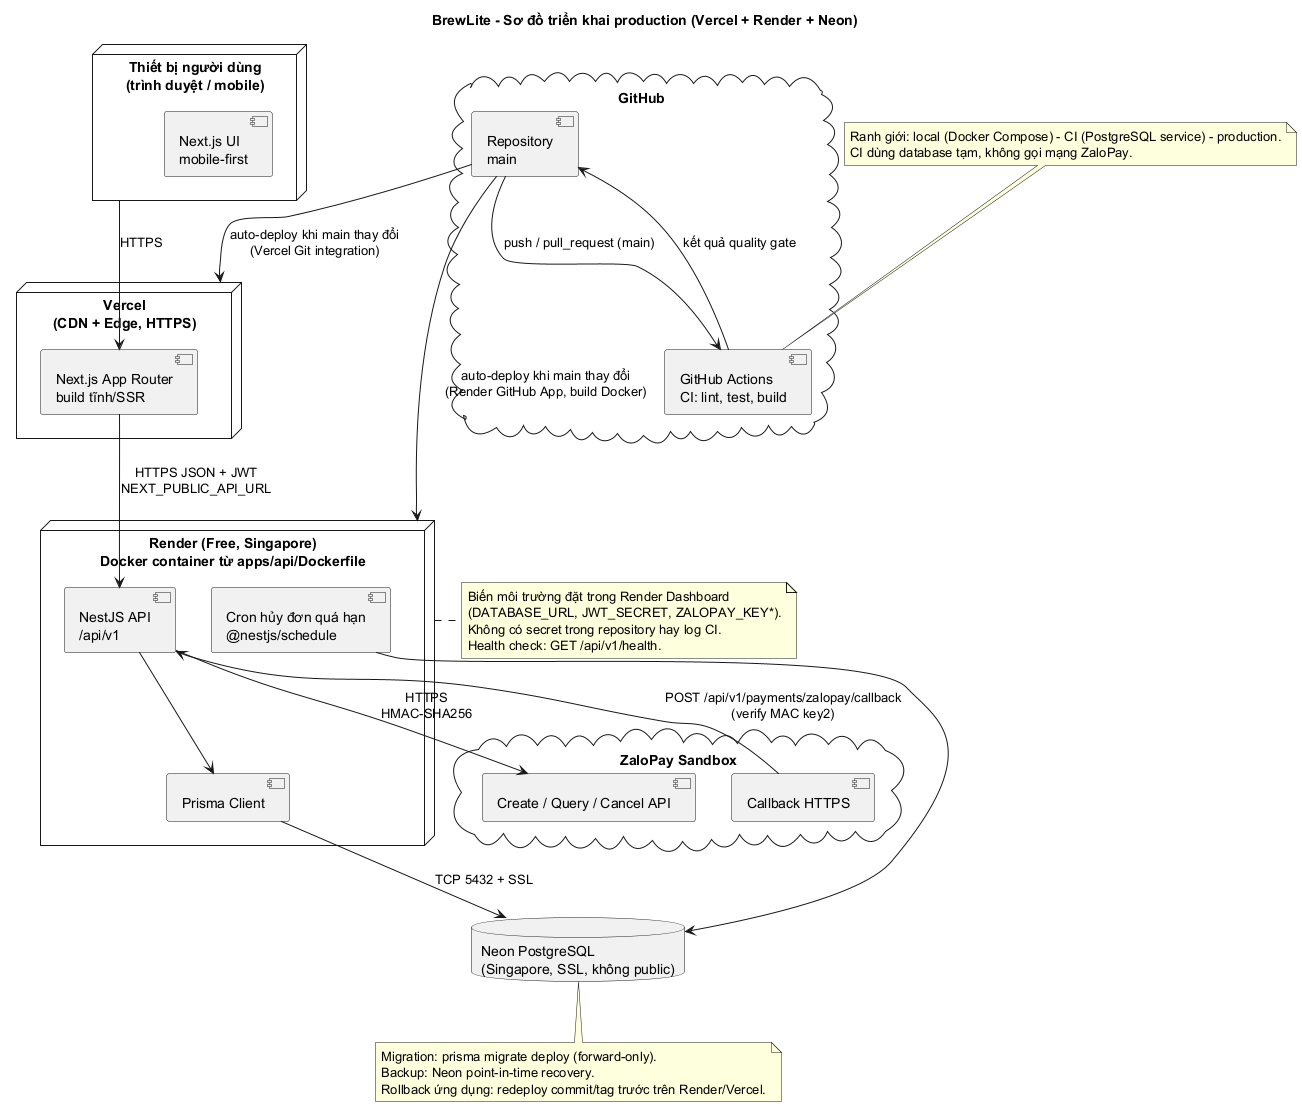
\includegraphics[width=0.68\textwidth]{../figures/diagrams/BrewLite-Deployment.png}
\caption{Sơ đồ triển khai: Vercel (web) -- Render (API) -- Neon (cơ sở dữ liệu) -- ZaloPay Sandbox}
\label{fig:deploy}
\end{figure}

\begin{table}[H]
\centering\small
\caption{Chín module nghiệp vụ của API}
\label{tab:modules}
\begin{tabularx}{\textwidth}{@{}l X@{}}
\toprule
\textbf{Module} & \textbf{Trách nhiệm} \\
\midrule
\code{auth} & Đăng ký, đăng nhập, cấp và kiểm tra JWT, chiến lược xác thực. \\
\code{users} & Hồ sơ người dùng, vai trò, danh sách khách hàng cho quản trị. \\
\code{products} & Thực đơn, danh mục, giá theo size, tìm kiếm và lọc. \\
\code{cart} & Giỏ hàng phía máy chủ và kiểm tra tồn kho trước khi đặt. \\
\code{orders} & Tạo đơn, máy trạng thái, huỷ đơn, lịch sử trạng thái. \\
\code{payments} & Tạo giao dịch ZaloPay, callback, truy vấn, đối soát, idempotency. \\
\code{ingredients} & Nguyên liệu, tồn kho, cảnh báo dưới định mức. \\
\code{recipes} & Định lượng nguyên liệu cho từng sản phẩm theo size. \\
\code{stock-imports} & Phiếu nhập kho và cập nhật tồn theo lô. \\
\bottomrule
\end{tabularx}
\end{table}

\section{Giao diện}
\label{sec:ui}

Toàn bộ ảnh dưới đây được chụp trực tiếp trên bản production ngày 15/11/2026, ở hai kích thước:
390$\times$844 (điện thoại) và 1440$\times$900 (máy tính để bàn).

\subsection{Khách hàng: xem thực đơn và chọn món}

\begin{figure}[H]
\centering
\shot{../figures/as2/view/01-menu-mobile.png}{Thực đơn, 8 món đang phục vụ}
\hfill
\shot{../figures/as2/view/02-chi-tiet-size-topping.png}{Chọn size và topping}
\hfill
\shot{../figures/as2/view/03-gio-hang-mobile.png}{Giỏ hàng, bước 1/3}
\caption{Luồng chọn món trên điện thoại: thực đơn, tuỳ chọn size/topping và giỏ hàng}
\label{fig:ui-menu}
\end{figure}

Thực đơn hiển thị đủ 8 món kèm ảnh, nhãn danh mục và giá khởi điểm; ô tìm kiếm lọc ngay khi gõ và
chấp nhận từ khoá không dấu. Hộp thoại chọn món cho phép đổi size, thêm topping và cập nhật tổng
tiền trước khi thêm vào giỏ. Giỏ hàng giữ nguyên khi tải lại trang nhờ lưu cục bộ, đồng thời hiển thị
bước hiện tại trong quy trình ba bước để người dùng biết mình đang ở đâu.

\subsection{Khách hàng: đăng nhập, đặt hàng và thanh toán}

\begin{figure}[H]
\centering
\shot{../figures/as2/view/04-dang-nhap-mobile.png}{Đăng nhập}
\hfill
\shot{../figures/as2/view/05-checkout-mobile.png}{Điểm và mã khuyến mãi}
\hfill
\shot{../figures/as2/view/06-thanh-toan-zalopay-mobile.png}{Chọn ZaloPay Sandbox}
\caption{Đăng nhập, áp dụng điểm tích luỹ và chọn phương thức thanh toán}
\label{fig:ui-checkout}
\end{figure}

Khi khách chưa đăng nhập mà bấm \emph{Tiến hành thanh toán}, hệ thống chuyển tới trang đăng nhập kèm
tham số quay lại, thay vì báo lỗi. Trang thanh toán cho thấy số điểm hiện có (120 điểm), hạn mức sử
dụng và số tiền dự kiến trước khi chuyển sang cổng thanh toán. Bước 3/3 ghi rõ đây là giao dịch thử
nghiệm, không dùng tiền thật.

\begin{figure}[H]
\centering
\shot{../figures/as2/view/07-tao-giao-dich-zalopay.png}{Liên kết sang ZaloPay}
\hfill
\shot{../figures/as2/view/08-lich-su-don-mobile.png}{Lịch sử đơn}
\hfill
\shot{../figures/as2/view/09-xac-nhan-don-mobile.png}{Chi tiết và trạng thái đơn}
\caption{Giao dịch được tạo thật trên ZaloPay Sandbox, lịch sử và chi tiết đơn hàng}
\label{fig:ui-zalopay}
\end{figure}

Sau khi bấm tạo thanh toán, API gọi ZaloPay và nhận về liên kết \code{openinapp} thật; trạng thái đơn
chuyển sang \emph{Chờ thanh toán} và trang tự cập nhật mỗi 15 giây. Lịch sử đơn hiển thị mã đơn, thời
điểm, số món, trạng thái và tổng tiền, kèm lối tắt tiếp tục thanh toán cho đơn còn chờ.

\subsection{Quản trị}

\begin{figure}[H]
\centering
\shot{../figures/as2/view/10-admin-dashboard-mobile.png}{Tổng quan}
\hfill
\shot{../figures/as2/view/11-admin-don-hang-mobile.png}{Đơn hàng}
\hfill
\shot{../figures/as2/view/12-admin-kho-nguyen-lieu-mobile.png}{Kho nguyên liệu}
\caption{Khu vực quản trị: tổng quan, đơn hàng và kho nguyên liệu}
\label{fig:ui-admin}
\end{figure}

Trang tổng quan gom số đơn, số đơn đã thanh toán, số sản phẩm đang bán và cảnh báo tồn kho dưới định
mức. Danh sách đơn cho phép chuyển trạng thái theo đúng quy trình. Trang kho hiển thị từng nguyên
liệu với tồn hiện tại, định mức tối thiểu và đơn vị tính.

\begin{figure}[H]
\centering
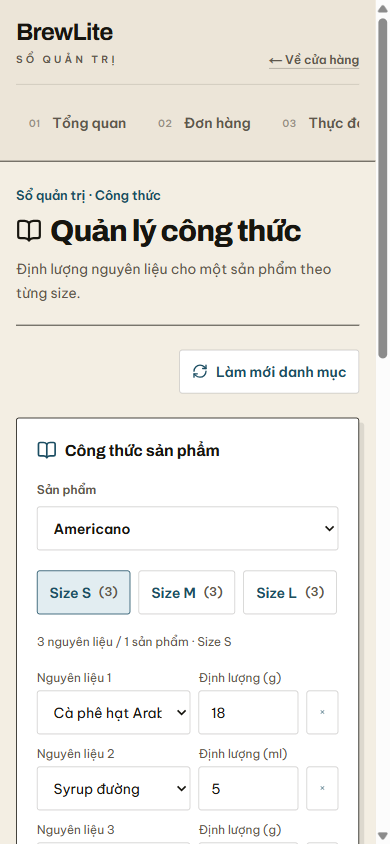
\includegraphics[width=0.30\textwidth]{../figures/as2/view/13-admin-cong-thuc-mobile.png}
\caption{Trang công thức: định lượng nguyên liệu cho một sản phẩm theo từng size}
\label{fig:ui-recipe}
\end{figure}

\begin{note}[Điểm đáng chú ý]
Mỗi dòng công thức gắn một nguyên liệu với một định lượng cụ thể cho từng size. Khi lưu, hệ thống kiểm
tra trùng nguyên liệu và chặn định lượng không hợp lệ; nhờ vậy cùng một sản phẩm có thể có định lượng
khác nhau ở size S, M và L mà vẫn giữ đúng một dòng cho mỗi cặp (sản phẩm, nguyên liệu, size).
\end{note}

\subsection{Giao diện máy tính để bàn}

\begin{figure}[H]
\centering
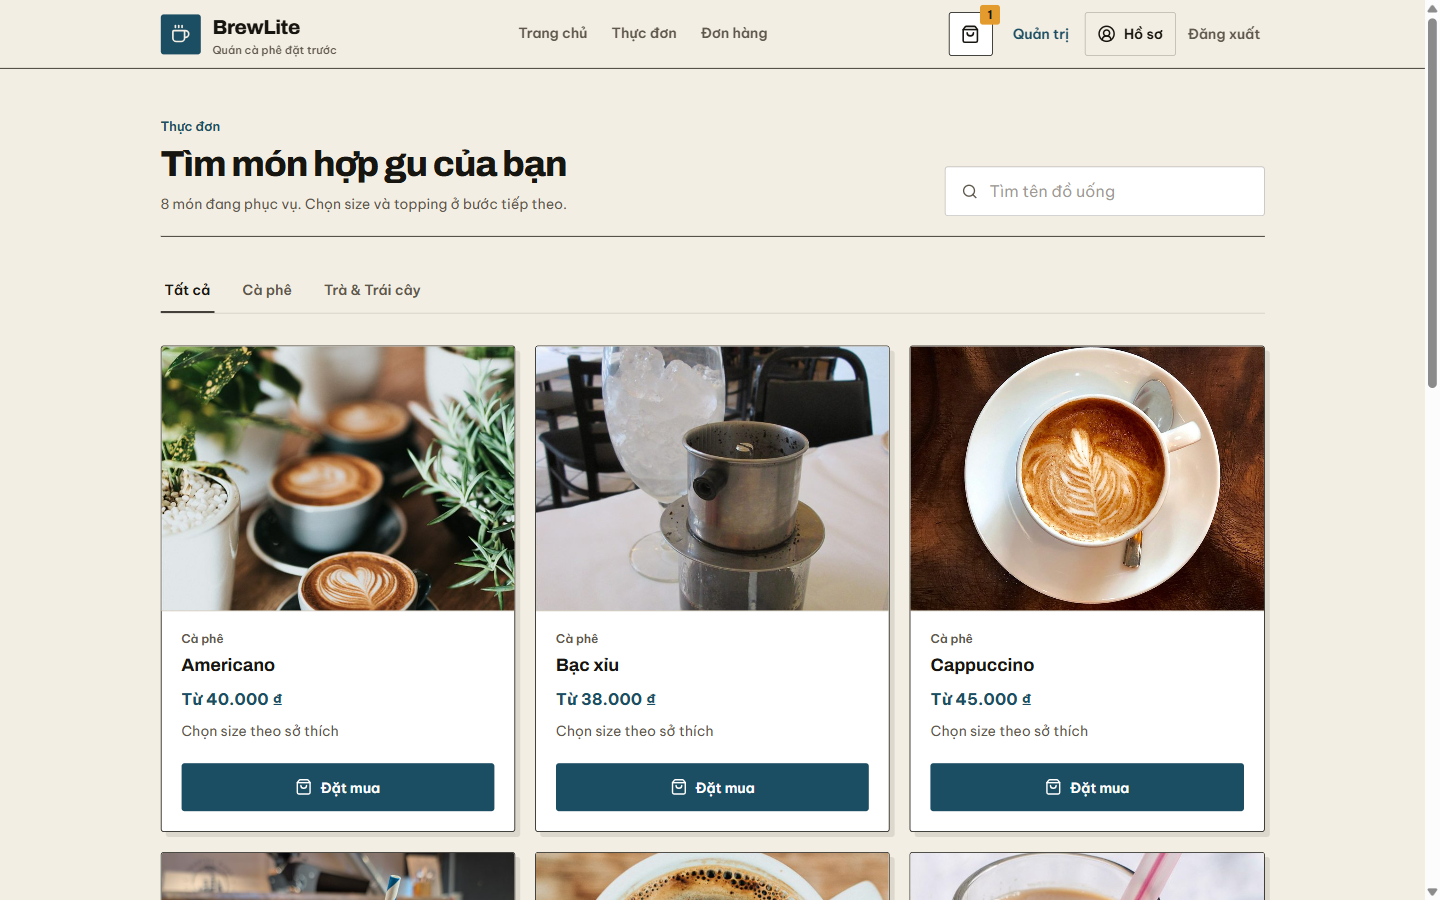
\includegraphics[width=0.94\textwidth]{../figures/as2/14-menu-desktop.png}
\caption{Thực đơn ở kích thước 1440$\times$900: bố cục lưới nhiều cột, giữ nguyên thứ tự ưu tiên}
\label{fig:ui-desktop}
\end{figure}

\begin{figure}[H]
\centering
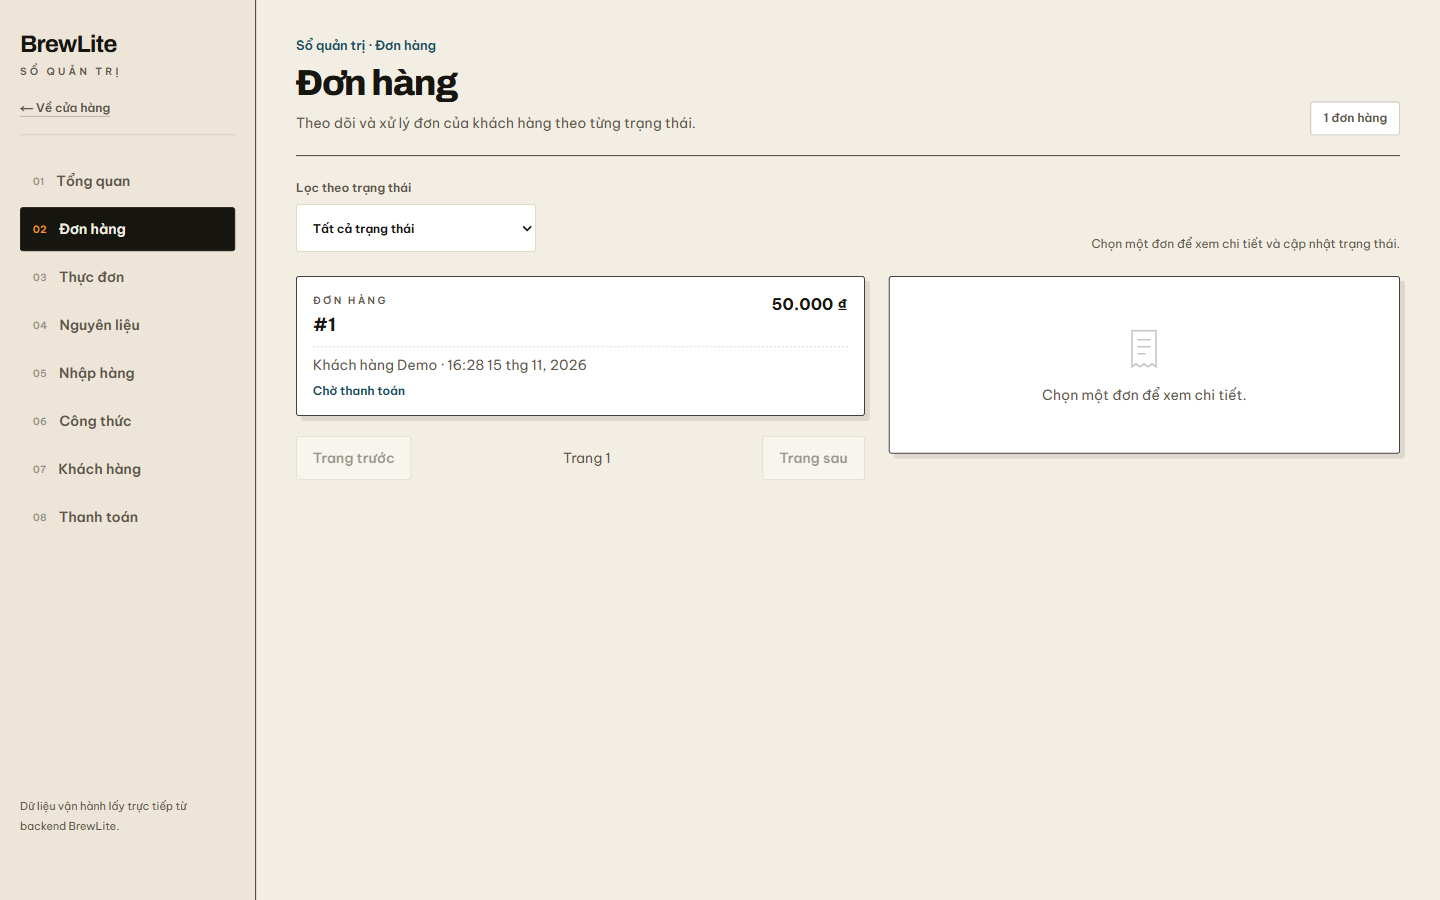
\includegraphics[width=0.94\textwidth]{../figures/as2/15-admin-don-hang-desktop.png}
\caption{Quản lý đơn hàng trên máy tính: bảng đơn, bộ lọc trạng thái và thao tác chuyển bước}
\label{fig:ui-admin-desktop}
\end{figure}

\begin{figure}[H]
\centering
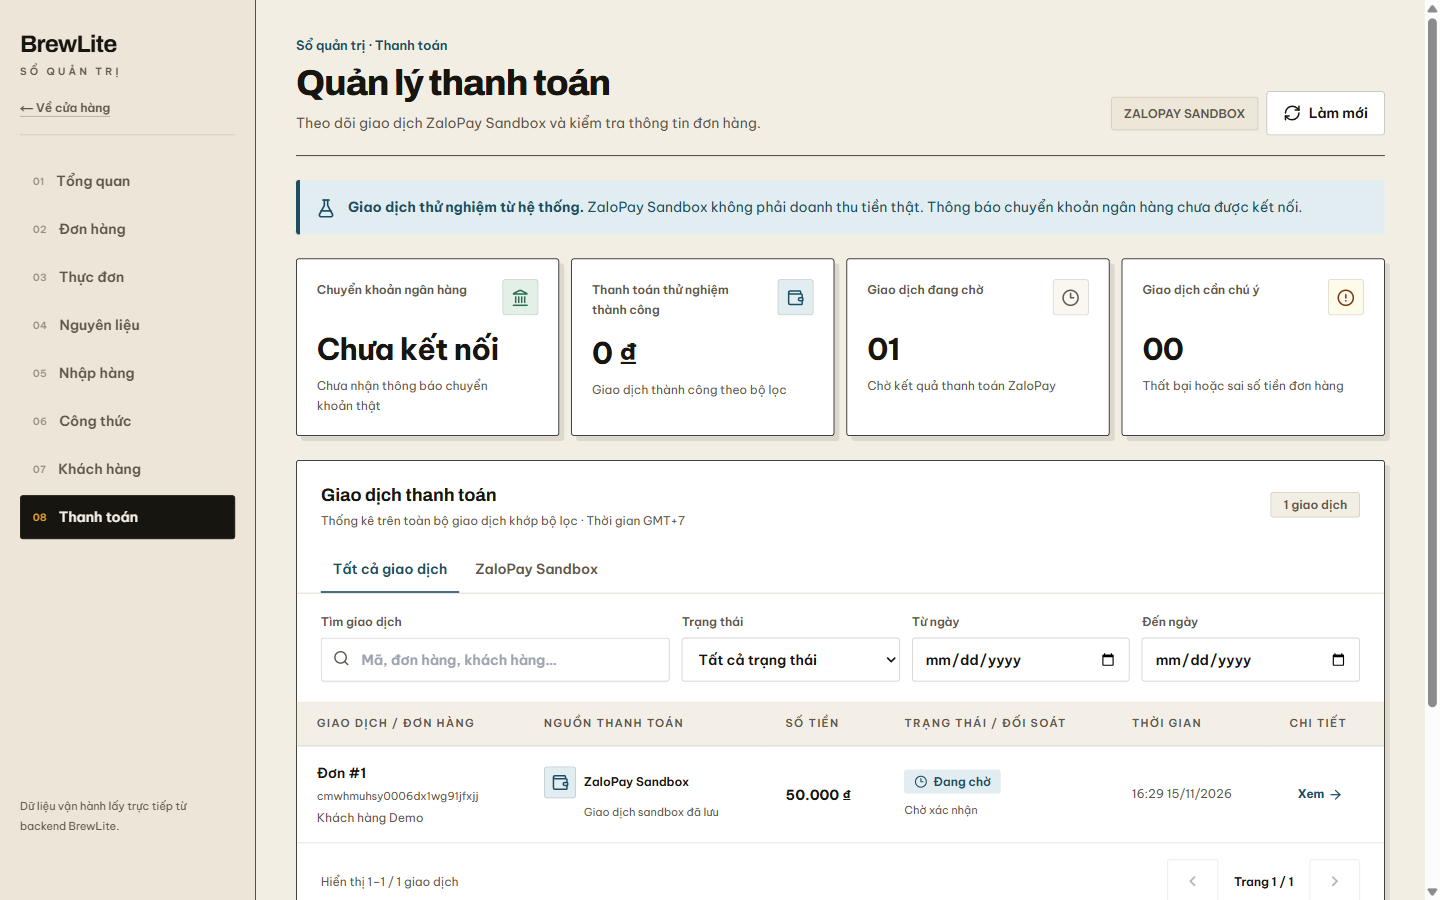
\includegraphics[width=0.94\textwidth]{../figures/as2/16-admin-thanh-toan-desktop.png}
\caption{Đối soát thanh toán: mã giao dịch, phương thức, trạng thái và số tiền}
\label{fig:ui-admin-pay}
\end{figure}

\section{Kiểm thử và chất lượng mã nguồn}

\subsection{Kiểm thử tự động}
Backend dùng \code{node:test} của Node.js (không dùng Jest hay Supertest) với 15 tệp kiểm thử; frontend
dùng cùng bộ chạy với 5 tệp. Các bài kiểm thử tích hợp chạy trên một schema PostgreSQL dùng một lần,
được tạo và xoá trong quá trình chạy, nên không phụ thuộc dữ liệu của môi trường phát triển.

\begin{table}[H]
\centering\small
\caption{Nhóm kiểm thử backend và phạm vi bao phủ}
\label{tab:tests}
\begin{tabularx}{\textwidth}{@{}p{4.6cm} X c@{}}
\toprule
\textbf{Nhóm} & \textbf{Nội dung kiểm chứng} & \textbf{Số tệp} \\
\midrule
Thực đơn và quyền truy cập & Danh sách sản phẩm, chi tiết, lọc, chặn truy cập trái phép. & 2 \\
Xác thực và hồ sơ & Đăng ký, đăng nhập, token hết hạn, cập nhật hồ sơ. & 1 \\
Giỏ hàng & Thêm, sửa, xoá, kiểm tra tồn kho trước khi đặt. & 1 \\
Đơn hàng & Tạo đơn, máy trạng thái, huỷ đơn, phân quyền quản trị. & 3 \\
Tồn kho và công thức & Trừ kho theo công thức, tranh chấp đồng thời, hoàn kho theo ảnh chụp. & 3 \\
Thanh toán & Tạo giao dịch, callback, idempotency, đổi phương thức thanh toán. & 2 \\
Khuyến mãi và giới hạn & Voucher, điểm tích luỹ, giới hạn tần suất yêu cầu. & 2 \\
Luồng tích hợp & Luồng đặt -- thanh toán -- huỷ xuyên nhiều module. & 1 \\
\bottomrule
\end{tabularx}
\end{table}

\begin{table}[H]
\centering\small
\caption{Kết quả chạy kiểm thử và kiểm tra chất lượng}
\label{tab:results}
\begin{tabularx}{\textwidth}{@{}l X l@{}}
\toprule
\textbf{Hạng mục} & \textbf{Lệnh} & \textbf{Kết quả} \\
\midrule
Kiểm thử backend & \code{npm test} (trong \file{apps/api}) & 49/49 đạt, 85,8 giây \\
Kiểm thử frontend & \code{npm test} (trong \file{apps/web}) & 10/10 đạt \\
Build backend & \code{npm run build} & Thành công \\
Build frontend & \code{npm run build} & Thành công, 21 tuyến đường \\
Lint frontend & \code{npm run lint} & 0 lỗi, 5 cảnh báo \\
\bottomrule
\end{tabularx}
\end{table}

Năm cảnh báo lint đều là cảnh báo nhẹ về phụ thuộc trong hook và biến chưa dùng; không có lỗi chặn
build. Backend chưa cấu hình ESLint riêng mà dựa vào trình biên dịch TypeScript strict và \code{nest
build} để phát hiện lỗi kiểu.

\subsection{Tích hợp liên tục}
Workflow \file{.github/workflows/ci.yml} chạy trên mỗi thay đổi của \code{main} và trên pull request:
cài phụ thuộc, sinh Prisma Client, chạy kiểm thử backend với PostgreSQL service, build và lint frontend.
Tính đến 15/11/2026, workflow đã chạy \textbf{16 lần trên \code{main}}: 13 thành công và 3 thất bại
trong giai đoạn phát triển; lần chạy gần nhất thành công. Dự án \textbf{chưa có workflow triển khai
tự động (CD)}: việc phát hành dựa trên tích hợp Git của Vercel và Render, kích hoạt khi \code{main}
thay đổi. Đây là khoảng trống được ghi nhận ở Mục~\ref{sec:limit}.

\subsection{Kiểm tra giao diện và lỗi hiển thị}
Mỗi màn hình được kiểm tra trên trình duyệt thật: tải lại trang, đăng nhập và đăng xuất, thêm món vào
giỏ, tạo giao dịch, chuyển trạng thái đơn ở trang quản trị. Kết quả:

\begin{table}[H]
\centering\small
\caption{Kết quả kiểm tra giao diện}
\label{tab:uicheck}
\begin{tabularx}{\textwidth}{@{}p{4.4cm} X p{1.7cm}@{}}
\toprule
\textbf{Hạng mục} & \textbf{Kết quả} & \textbf{Đánh giá} \\
\midrule
Cuộn ngang ở 390 px & Kiểm tra 8 tuyến đường (\code{/menu}, \code{/cart}, \code{/login},
\code{/orders}, \code{/checkout}, \code{/admin}, \code{/admin/recipes}, \code{/admin/orders}): không
có tràn ngang. & \pass \\
Cuộn ngang ở 1440 px & Kiểm tra 5 tuyến đường: không có tràn ngang. & \pass \\
Ảnh và biểu tượng & Không có ảnh vỡ; ảnh sản phẩm tải từ Unsplash có thuộc tính thay thế. & \pass \\
Trạng thái rỗng và lỗi & Giỏ rỗng, đơn rỗng, kho rỗng đều có thông điệp hướng dẫn thay vì màn hình trắng. & \pass \\
Lỗi console & Còn hai lỗi: \code{favicon.ico} trả 404 và \code{/auth/me} trả 401 khi chưa đăng nhập. & \partialok \\
\bottomrule
\end{tabularx}
\end{table}

Hai lỗi console nêu trên không ảnh hưởng tới chức năng nhưng vẫn là điểm cần sửa: thiếu tệp biểu tượng
ở thư mục công khai, và lời gọi kiểm tra phiên chạy ngay cả khi người dùng chưa đăng nhập. Cả hai đã
được ghi vào danh sách việc cần làm kèm cách khắc phục cụ thể.

\section{Đo hiệu năng}
\label{sec:perf}

\subsection{Phương pháp}
Ba endpoint đọc dữ liệu mẫu được gọi 5 lần liên tiếp, cách nhau 300 ms, từ một máy khách tại Việt Nam
tới API trên Render (Singapore) qua HTTPS. Thời gian đo là thời gian phản hồi đầy đủ của yêu cầu
HTTP, bao gồm cả độ trễ mạng. Trước khi đo, API đã được đánh thức để loại bỏ ảnh hưởng của cơ chế
ngủ đông.

\begin{table}[H]
\centering\small
\caption{Kết quả đo thời gian phản hồi (đơn vị: mili giây)}
\label{tab:perf}
\begin{tabular}{@{}l rrrrr rrr c@{}}
\toprule
\textbf{Endpoint} & \textbf{L1} & \textbf{L2} & \textbf{L3} & \textbf{L4} & \textbf{L5}
& \textbf{Nhỏ nhất} & \textbf{Trung vị} & \textbf{Lớn nhất} & \textbf{Kết luận} \\
\midrule
\code{/health}      & 96  & 99  & 96  & 133 & 95  & 95  & 96  & 133 & \pass \\
\code{/products}    & 116 & 185 & 165 & 182 & 194 & 116 & 182 & 194 & \pass \\
\code{/products/:id}& 104 & 89  & 81  & 80  & 81  & 80  & 81  & 104 & \pass \\
\bottomrule
\end{tabular}
\end{table}

Cả ba endpoint đều đạt ngưỡng NFR-01 (dưới 500 ms) với biên an toàn lớn: trường hợp xấu nhất là
194 ms, chưa bằng 40\% ngưỡng. Endpoint danh sách có thời gian cao hơn vì trả về 8 sản phẩm kèm bảng
giá theo size và thông tin danh mục.

\subsection{Khởi động nguội}
Lần gọi đầu tiên sau một khoảng thời gian không có lưu lượng mất \textbf{52.483 ms} (khoảng 52 giây)
do Render ở gói miễn phí tạm dừng dịch vụ khi rảnh. Đây là giới hạn của hạ tầng, không phải của mã
ứng dụng: sau khi dịch vụ thức, mọi phản hồi đều dưới 200 ms. Ba hướng xử lý đã được ghi nhận: nâng
gói Render để tắt chế độ ngủ, dùng bộ hẹn giờ gọi \code{/health} định kỳ, hoặc chuyển sang nền tảng
không tạm dừng dịch vụ.

\section{Quy trình phát triển và đóng góp}

\subsection{Các sprint}
Lịch sử commit được chia thành ba giai đoạn dựa trên mốc thời gian thực tế của kho mã:

\begin{table}[H]
\centering\small
\caption{Phân kỳ phát triển theo lịch sử commit}
\label{tab:sprint}
\begin{tabularx}{\textwidth}{@{}l l c X@{}}
\toprule
\textbf{Giai đoạn} & \textbf{Thời gian} & \textbf{Số commit} & \textbf{Nội dung chính} \\
\midrule
Sprint 1 & 20/10 -- 26/10/2026 & 49 & Khung monorepo, lược đồ cơ sở dữ liệu, xác thực, thực đơn,
giỏ hàng. \\
Sprint 2 & 27/10 -- 03/11/2026 & 5 & Ổn định luồng đặt hàng, sửa lỗi phát hiện khi tích hợp. \\
Sprint 3 & 04/11 -- 14/11/2026 & 40 & Kho nguyên liệu và công thức, thanh toán ZaloPay, quản trị,
kiểm thử, tài liệu và triển khai. \\
\bottomrule
\end{tabularx}
\end{table}

\subsection{Phân công theo module}
Nhóm chia việc theo module thay vì theo tầng, để mỗi thành viên chịu trách nhiệm trọn vẹn từ dữ liệu
tới giao diện của phần mình. Bảng~\ref{tab:contrib} tóm tắt phạm vi và bằng chứng.

\begin{table}[H]
\centering\footnotesize
\caption{Phân công P1--P6 theo module và bằng chứng trong kho mã}
\label{tab:contrib}
\begin{tabularx}{\textwidth}{@{}p{1.0cm} p{2.3cm} X@{}}
\toprule
\textbf{Vai trò} & \textbf{Module phụ trách} & \textbf{Bằng chứng chính} \\
\midrule
P1 & Kiến trúc, đơn hàng, thanh toán, cơ sở dữ liệu, triển khai &
\file{orders/}, \file{payments/}, \file{schema.prisma}, migration, \file{order-state.ts}, workflow CI,
cấu hình Vercel/Render, tài liệu trong \file{docs/}. \\
P2 & Thực đơn và danh mục phía web & \file{app/menu/}, \file{lib/menu-filter.ts},
\file{services/product.service.ts}. \\
P3 & Chi tiết sản phẩm và tuỳ chọn & \file{app/products/[id]/}, \file{product-purchase-modal.tsx},
\file{types/product.ts}. \\
P4 & Giỏ hàng, kho, công thức & \file{cart/}, \file{ingredients/}, \file{recipes/},
\file{stock-imports/}, bộ điều khiển đơn hàng cho quản trị. \\
P5 & Xác thực, người dùng, tích hợp ZaloPay & \file{auth/}, \file{jwt.strategy.ts}, \file{users/},
các tệp \file{payments/zalopay-*}. \\
P6 & Kiểm thử và chất lượng & 15 tệp kiểm thử backend, 5 tệp frontend, kịch bản kiểm thử đầu cuối,
theo dõi lỗi giao diện. \\
\bottomrule
\end{tabularx}
\end{table}

\subsection{Quy trình làm việc}
Công việc được theo dõi bằng pull request trên GitHub: mỗi nhánh gắn với một phạm vi thay đổi, mô tả
pull request nêu rõ phần đã làm và cách kiểm chứng. Kho mã có 19 pull request, trong đó 16 đã được
hợp nhất vào \code{main}. Nhóm \textbf{không sử dụng Jira, Trello hay Figma}: yêu cầu và thiết kế được
ghi trực tiếp trong \file{docs/} (đặc tả yêu cầu, thiết kế cơ sở dữ liệu, ma trận truy vết, quyết định
kiến trúc) và trong mô tả pull request, nên mọi quyết định đều truy vết được từ commit.

\section{Hạn chế và hướng phát triển}
\label{sec:limit}

\begin{itemize}
  \item \textbf{Chưa có quy trình triển khai tự động.} Vercel và Render tự build khi \code{main} thay
        đổi, nhưng chưa có workflow CD trong GitHub Actions, chưa có bước kiểm thử khói sau khi phát
        hành và chưa có cơ chế tự động quay lui.
  \item \textbf{Khởi động nguội kéo dài.} Gói miễn phí của Render tạm dừng dịch vụ khi rảnh, khiến lần
        truy cập đầu tiên mất khoảng 52 giây. Cần nâng gói hoặc duy trì nhiệt cho dịch vụ.
  \item \textbf{Kiểm thử giao diện chưa tự động.} Các kịch bản trình duyệt hiện được chạy thủ công;
        chưa có Playwright/Cypress trong CI, nên hồi quy giao diện chỉ được phát hiện khi có người
        kiểm tra.
  \item \textbf{Còn lỗi console nhỏ.} Thiếu biểu tượng trang và lời gọi kiểm tra phiên khi chưa đăng
        nhập; cả hai đã có cách khắc phục nhưng chưa phát hành.
  \item \textbf{Phạm vi nghiệp vụ còn hẹp.} Chưa hỗ trợ giao hàng, nhiều chi nhánh, hoá đơn điện tử và
        ứng dụng di động native.
  \item \textbf{Chưa có công cụ thiết kế chuyên dụng.} Nhóm không dùng Figma; giao diện được thiết kế
        trực tiếp bằng mã nguồn, nên thiếu bản đặc tả hình ảnh độc lập để so sánh.
\end{itemize}

Hướng tiếp theo ưu tiên bốn việc: bổ sung workflow CD kèm kiểm thử khói và quay lui, đưa kiểm thử
trình duyệt vào CI, xử lý hai lỗi console còn lại, và nâng cấu hình hạ tầng để loại bỏ khởi động nguội.

\section*{Tài liệu tham khảo}
\addcontentsline{toc}{section}{Tài liệu tham khảo}
\begin{enumerate}[label={[\arabic*]},leftmargin=2.2em]
  \item NestJS Documentation. \url{https://docs.nestjs.com}. Truy cập 15/11/2026.
  \item Next.js Documentation (App Router). \url{https://nextjs.org/docs}. Truy cập 15/11/2026.
  \item Prisma ORM Documentation. \url{https://www.prisma.io/docs}. Truy cập 15/11/2026.
  \item ZaloPay Payment Gateway -- Sandbox API. \url{https://docs.zalopay.vn}. Truy cập 15/11/2026.
  \item OWASP Application Security Verification Standard. \href{https://owasp.org/www-project-asvs/}{owasp.org/www-project-asvs}.
        Truy cập 15/11/2026.
  \item Node.js Test Runner Documentation. \url{https://nodejs.org/api/test.html}. Truy cập 15/11/2026.
\end{enumerate}

\end{document}





